\documentclass[preview]{standalone}

\usepackage{amsmath}
\usepackage{amssymb}
\usepackage{stellar}
\usepackage{bettelini}

\hypersetup{
    colorlinks=true,
    linkcolor=black,
    urlcolor=blue,
    pdftitle={Biologia},
    pdfpagemode=FullScreen,
}

\begin{document}

\title{Biologia}
\id{biologia-genetica}
\genpage

\begin{snippetdefinition}{locus-genetico-definizione}{Locus genetico}
    Con \textit{locus genetico} si intende si intende una posizione fissata per
    un certo gene nel cromosoma.
\end{snippetdefinition}

\begin{snippet}{alleri-expl}
    Le varianti di un gene si chiamano \textbf{alleri}, i quali possono essere uguali o diversi
    (es. occhi marroni-verdi etc.). Per ogni gene vi sono 2 alleri, siccome vi è una coppia di cromosomi omologhi.
\end{snippet}

\begin{snippetdefinition}{cromatina-definizione}{Cromatina}
    la \textit{cromatina} è il DNA composta da 46 cromosomi singoli non spiralizzati (formano un groviglio).
\end{snippetdefinition}

\begin{snippet}{f1a85dd0-75f5-45a9-8bdc-4651a9accf8e}
    Durante la duplicazione del DNA, all'interno della cromatina,
    alcuni enzimi duplicano tutti i cromosomi.
    I 92 cromosomi nella cromatina vengono separati correttamente, rimanendo non spiralizzati.
    Successivamente i cromosomi si spiralizzando su delle proteine formando una struttura spiralizzata ad X.
\end{snippet}

% immagine

\begin{snippetdefinition}{cromatidi-definizione}{Cromatidi}
    I \textit{cromatidi} sono le braccia di un cromosoma X.
    Un cromosoma X ha quindi 2 cromatidi fratelli (destra e sinistra).
\end{snippetdefinition}

\plain{La mitosi consiste nel separare i cromatidi fratelli, e quindi duplicare l'informazione,
ottendo due cromosomi singoli spiralizzati.}

\begin{snippetdefinition}{cariotipo-definizione}{Cariotipo}
    Con \textit{cariotipo} si intende l'insieme di tutti le 23 coppie di cromosomi.
\end{snippetdefinition}
% rivedere Def

\begin{snippet}{autosomi-expl}
    Gli ultimi due cromosomi sono quelli che determinano il sesso (cromosomi sessuali),
    mentre gli altri si chiamano \textbf{autosomi}.
\end{snippet}

\begin{snippet}{cariotipo-expl}
    \begin{center}
    \begin{figure}[ht]
        \centering
        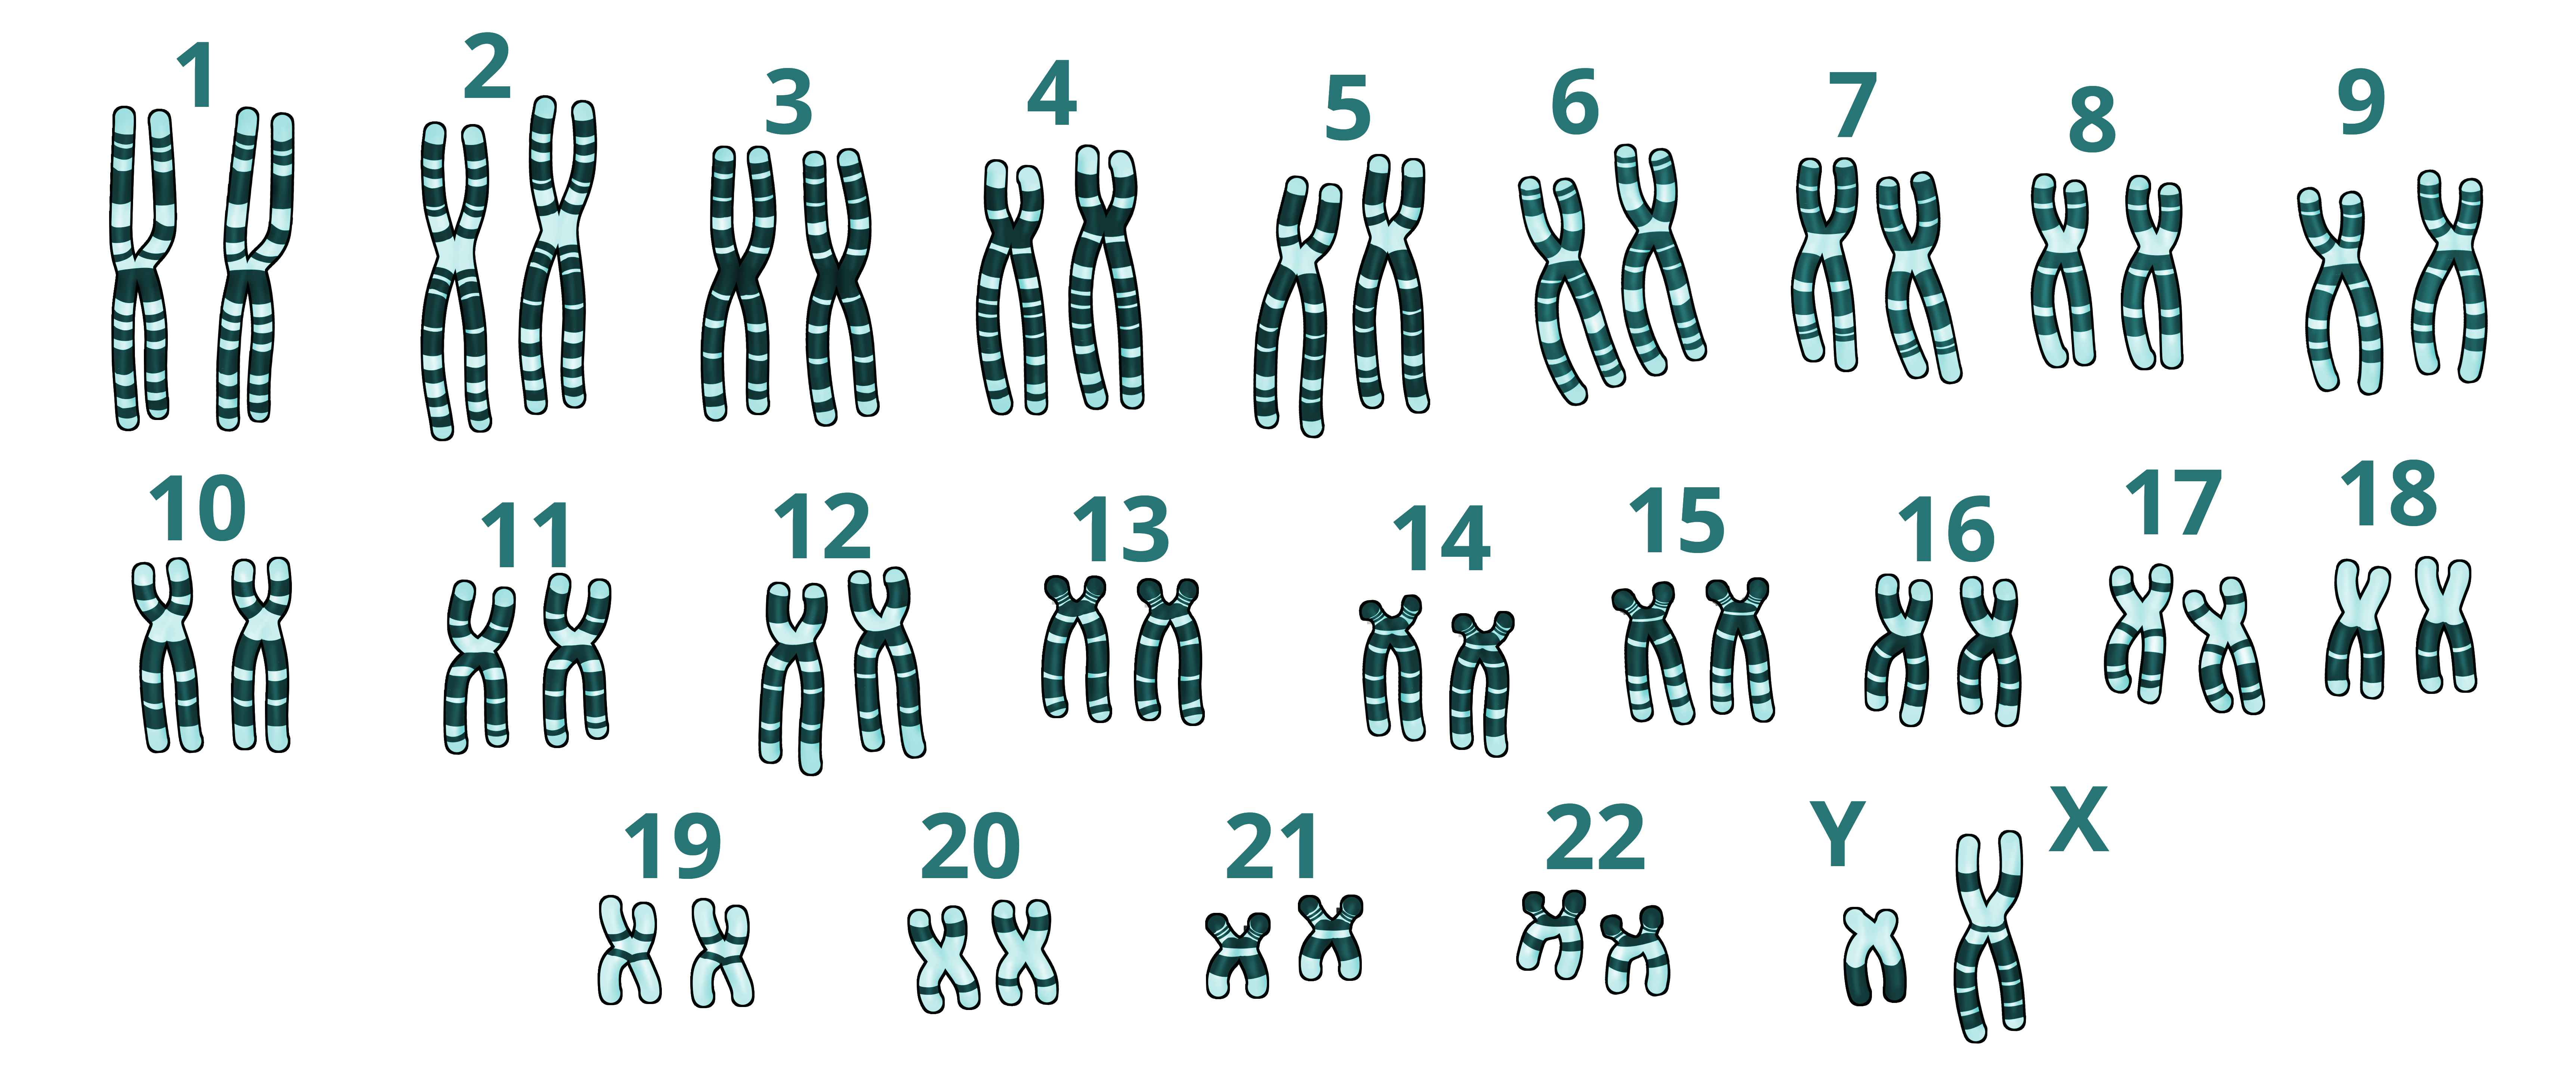
\includegraphics[width=0.8\textwidth]{./resources/cariotipo}
    \end{figure}
    \end{center}
\end{snippet}

\end{document}